\section{Fourier Neural Operators and Neural Networks}
The FVM, together with other numerical solvers such as the FDM and FEM (Finite Element Method), solves PDEs by discretizing the domain into a grid.
The finer the grid, the more accurate the solution, but also the more computationally expensive the solution. This introduces a trade-off between accuracy and computational cost.
Complex PDEs often require a fine grid to capture the solution accurately, which can be computationally expensive.
The hope for data-driven methods is that, by learning the dynamics of the solution, we can reduce the computational cost of solving PDEs and still maintain a high level of accuracy.
A classical neural network (NN), is able to learn a map from input to output, i.e., a map between finite-dimensional spaces.
Fourier Neural Operators stands out at they are able to learn mappings between function spaces, meaning they are also grid-independent.
The neural operator requires data only, and not the PDE itself.
This is obiviously a great advantage, if we are aiming to describe systems where the PDE is unknown. 
The neural operator is also able to transfer solutions between meshes, meaning that we can train the model on a coarse grid and transfer the solution to a fine grid, depending on the desired accuracy.
This is also referred to as the zero-shot super-resolution property.
We make the neural operator to a fourier neural operator, by using a fourier integral operator in the neural network.
We utilize the fact that differentation with respect to time is equivalent to multiplication in the Fourier domain.
(Not to be confused with the convolution theorem).

Another issue we are facing in this project is non-linearities.
Standard neural networks uses combinations of linear multiplications and non-linear activation functions to approximate non-linear functions.
Whereas, neural operators approximate non-linear operators, by combining linear functions and non-linear activation functions with global integral operators. 

\subsection{Convolutional Neural Networks}
Some text about CNNs.


\subsection{Fourier Neural Operators}
In this section, we will introduce the concept of Fourier Neural Operators (FNO).
The theory and method described here is based on the paper~\cite{FNO_2021}.

We consider the operator $G: A \to U$, that maps from a infinite-dimensional function space $A$ to another infinite-dimensional function space $U$.
We aim to approximate the exact operator $G$ by constructing the map
\begin{align*}
    G_{\theta}: A \mapsto U, \quad \theta \in \Theta,
\end{align*} 
where $\Theta$ is a finite-dimensional parameter space.
Consider the functions $a \in A$ and $u \in U$.
We can access the data by point wise evaluations of the functions, i.e., we have access to the observations ${\{a_j, u_j \}}_{j=1}^N$, in a domain $D \subset \mathbb{R}^d$, which is bounded open set.
The neural operator is iterative, where the update $v_t \mapsto v_{t+1}$ is defined as
\begin{align}
    v_{t+1}(x) := \sigma \left( W v_t(x) + \left( \mathcal{K}(a;\phi)v_t \right) (x) \right), \quad \forall x \in D
\end{align}
where $W: \mathbb{R}^{d_v} \to \mathbb{R}^{d_v}$ is a linear transformation, and $\sigma: \mathbb{R} \to \mathbb{R}$ is a non-linear activation function.
We define the Fourier integral operator $\mathcal{K}$ as 
\begin{align}
    \left( \mathcal{K}(\phi)v_t \right) (x) = \mathcal{F}^{-1} \left( R_{\phi} \cdot (\mathcal{F}v_t ) \right)(x), \quad \forall x \in D
\end{align}
where $\mathcal{F}$ is the Fourier transform, $\mathcal{F}^{-1}$ is the inverse Fourier transform, and $R$ is the linear transformation applied on the lower Fourier modes. 
We aim for a multi-step prediction model, which can predict a given number of time steps.

The network for the FNO model is illustrated in \autoref{fig:fourier_neural_network}.
\begin{figure}[H]
    \centering
    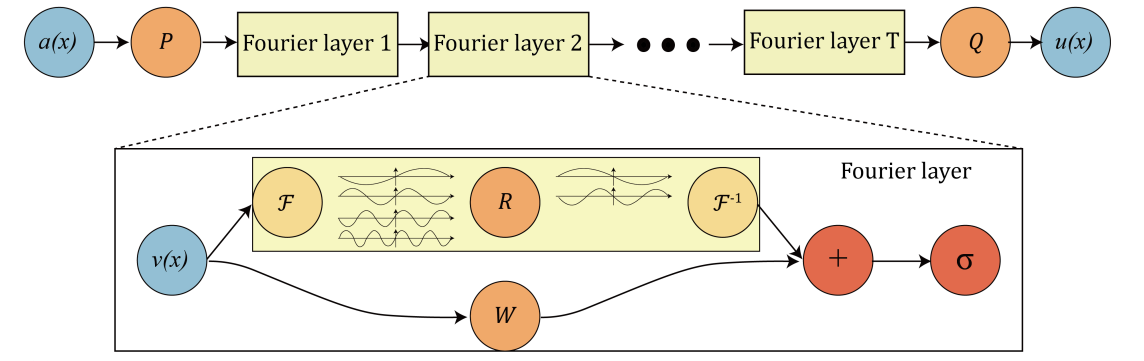
\includegraphics[width=0.7\textwidth]{C:/Users/Matteo/Shallow-Water-Equations/figs/fourier_neural_network.png}
    \caption{An overview of the network architecture with several Fourier layers. Illustration from~\cite{FNO_2021}.}\label{fig:fourier_neural_network}
\end{figure}
From the figure we see that the network consists of a input layer $P$, several Fourier layers and a output layer $Q$.
A Fourier layer consists of two parallel paths. The top path consists of a Fourier transformation $\mathcal{F}$, a linear transformation $R$ to filter out the higher Fourier modes, and a inverse Fourier transformation $\mathcal{F}^{-1}$.
The bottom path consists of a linear transformation $W$. 
The paths meet and there are applied an activation function $\sigma$.



Input-output mapping:
\begin{align*}
    \begin{bmatrix}
        a_0 \\
        a_1 \\
        \vdots \\
        a_{N-1}
    \end{bmatrix}
    \to
    \begin{bmatrix}
        u_0 \\
        u_1 \\
        \vdots \\
        u_{N-1}
    \end{bmatrix}
\end{align*}







